In this section, experiment setups and the results of each experiment in each step are discussed. Besides, different ideas and algorithms which are described in section \ref{sec:exp} are evaluated. At first, machine-learning-based experiments are presented. As machine learning feature engineering, requires multiple experiments to find best working predictors, there are many trials and errors for a variety of algorithms and ideas. Then, Deep learning models are compared to machine learning models. Finally, the FakeNews model is evaluated depends on best stance detection models.

The headline of news is a summary of its body content and most of the time, it carries valuable data. So, we focused on detecting the news headlines stance towards claim(H2C), as well as the news articles stance towards a claim(B2C). According to the lower amount of text in the news headline, most of the experiments are firstly applied to H2C. Then, better approaches are applied to A2C.  


\section{Dataset}
\label{sec:dataset}
The first Persian stance detection dataset (\cite{stance_persian})  is used in this project. \cite{stance_persian} dataset can be used in stance detection, summarization, and fake news detection tasks. This dataset contains 2124 news articles that cover information about 534 claims. Number of samples in each class is specified in table \ref{tbl:sdatapie}. Claims are retrieved from Shayeaat \footnote{shayeaat.ir} and Fakenews\footnote{fakenews.ir} websites. Each sample contains 3 different labels for the stance detection task, containing the article's headline toward the claim, the article's body toward the claim, and the article's headline toward its body. Samples are tagged manually. Four following classes are considered for stance classifying:
\begin{itemize}
	\item {\color{green!70!black}\textbf{Agree:}} The article clearly states that the claim is True without any ambiguity or amphibology. 
	\item {\color{red!70!black}\textbf{Disagree:}} The article clearly refutes that the claim without any ambiguity or amphibology. 
	\item {\color{yellow!70!black}\textbf{Discuss:}} The article contains information about the claim but doesn't have any evaluation of its truth. 
	\item {\color{gray!}\textbf{Unrelated:}} There isn't any information about the claim in the article.
\end{itemize}
Dataset samples distribution in each class is illustrated in Figure \ref{fig:datacom}. According to Figure \ref{fig:datacom}, the ratio of \textit{Agree}. Besides, \textit{Disagree} labels are much lower than the others and there is a potential risk for models to be biased on \textit{Unrelated} and \textit{Discuss}. Also, the percentage of \textit{Unrelated} label is higher in headline to claim than article to claim. A headline can be considered as a summary of news body. So, unlike news text, news headline may not have enough information to evaluate a claim.  Moreover, ratio of \textit{Discuss} to \textit{Agree} and \textit{Disagree} is higher in Article to claim in comparison to headline to claim. Accordingly, it seems that news agencies choose more controversial headlines to appeal reader's attention.

Furthermore, this dataset covers each claim veracity according to related news articles. Veracity labels statistics (FakeNews Dataset) is illustrated in table \ref{tbl:fakedata}. In this dataset, the main focus has been on published fake news, this can be inferred from figure \ref{fig:fake}. Three following labels are also considered for classifying news veracity for each claim-headline and claim-body pairs.

\begin{itemize} 
	\item {\color{green!70!black}\textbf{True:}} Reliable news agencies have asserted that this claim is a fact.
	\item {\color{red!70!black}\textbf{False:}} Unreliable news agencies have spread data about this claim and reliable news agencies have considered this claim as hearsay.
\item {\color{gray}\textbf{Unknown:}} There isn't enough integrity between reliable news agencies sources.
\end{itemize}




\begin{table}
	\centering
	\caption{Stance class distribution}
	\setlength{\extrarowheight}{5pt}
	\begin{tabularx}{1\textwidth} { 
			| >{\centering\arraybackslash}X 
			| >{\centering\arraybackslash}X 
			| >{\centering\arraybackslash}X 
			| >{\centering\arraybackslash}X 
			| >{\centering\arraybackslash}X | }
		\hline
		Label & Agree & Disagree & Unrelated & Discuss \\
		\hline \hline
		Headline to claim & 628  & 210  & 932 & 824  \\
		\hline
		Article to claim & 189  & 374  & 797 & 1196  \\
		\hline
		
	\end{tabularx} 
	\label{tbl:sdatapie}
\end{table}

\begin{figure}%
	\centering
	\subfloat[\centering Artcile to Claim]{{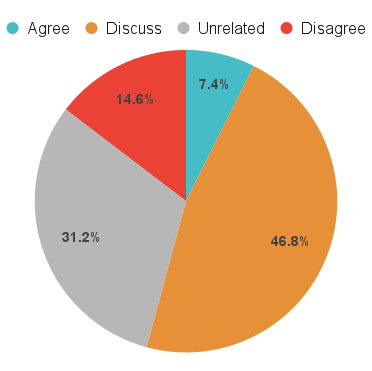
\includegraphics[width=6cm]{statistics/stance/a2c.png} }}%
	\qquad
	\subfloat[\centering Headline to claim ]{{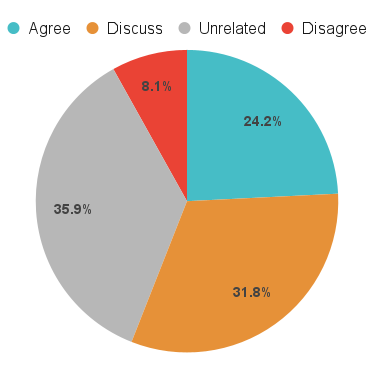
\includegraphics[width=6cm]{statistics/stance/h2c.png} }}%
	\caption{Comparison between Article to claim and Headline to claim labels, samples distribution in \cite{stance_persian} dataset.}%
	\label{fig:datacom}%
\end{figure}

\begin{table}
	\centering
	\caption{Fake news data set statistics}\label{fake-news-dataset}
	\small
	\setlength{\extrarowheight}{5pt}%
	\begin{tabularx} {0.7\textwidth}{ 
			| >{\centering\arraybackslash}X 
			| >{\centering\arraybackslash}X 
			| >{\centering\arraybackslash}X 
			| >{\centering\arraybackslash}X | }
		\hline 
		{\bf Used case}      & {\bf True} & {\bf False} & {\bf Unknown} \\ \hline  \hline
		{Test set}     &      {20}      &      {250}      &  {8} \\ 
		\hline
		{Training set}    &     {91}      &      {1003}       &   {35}\\
		\hline
			{Overall}    &     {111}      &      {1253}       &   {43}\\
		\hline
	\end{tabularx}
	\label{tbl:fakedata}
\end{table}

\begin{figure}%
	\centering
	{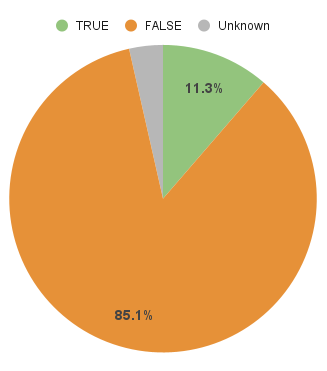
\includegraphics[width=5.5cm]{statistics/stance/fake.png} }
	\caption{Claim veracity label's distribution in \cite{stance_persian} dataset.}%
	\label{fig:fake}%
\end{figure}
  



\section{Tokenizetion}
Tokenization of \textit{Hazm}, \textit{Stanza}, \textit{NLTK}, and \textit{WordPiece} are evaluated against each other manually. Every single difference in each algorithm performance is evaluated\footnote{All different cases during corpus tokenization by those 4 algorithms are gathered in \href{https://docs.google.com/document/d/1SlRBnoyLntLJ5yalWXZ1EqJ0wRj4DyiEMJdewkEkrTM/edit?usp=sharing}{here}}. Only three cases are presented as examples to compare each tokenizer's performance in figure \ref{fig:tekenres}. As we need to remove particular words and patterns from the corpus,  it is important to find a tokenizer that distinguishes all words correctly. Besides, it shouldn't lose information while tokenizing and be as fast as possible. 

In figure \ref{fig:tekenres}, unsuitable tokens are highlighted in blue. There isn't any flawless algorithm. WordPiece is subwords based so there are some UNK tokens and words are wrongly broken. For example figure \ref{fig:tekenres}, part (b) blue highlighted word is broken into two pieces wrongly. Considering connected pronouns individually is the strength of \textit{Stanza} tokenizer. But sometimes the \text{Stanza} wrongly breaks an original word with a wrong assumption that the desired word has a connected pronoun. Figure \ref{fig:tekenres}, part (c) is a sample on wrong separating pronoun and at part (b), pronouns are separated correctly. It can be seen in figure \ref{fig:tekenres} \textit{Hazm}'s performance is highly similar to \textit{NLTK}. The only difference is that in contrast to \textit{NLTK}, Hazm separates numbers and punctuation in the corpus (Figure \ref{fig:tekenres}, part (a)). 

\begin{figure}%
	\centering
	\subfloat[\centering]{{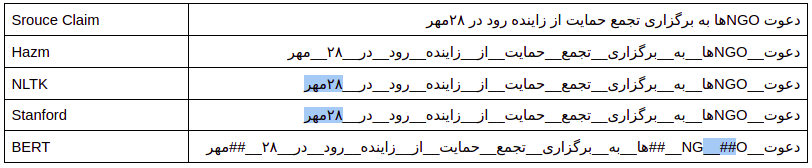
\includegraphics[width=16cm]{statistics/tokenizer/1.png} }}%
	\qquad
	\subfloat[\centering ]{{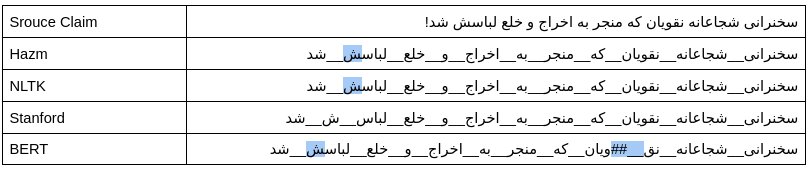
\includegraphics[width=16cm]{statistics/tokenizer/2.png} }}%
	\qquad
	\subfloat[\centering]{{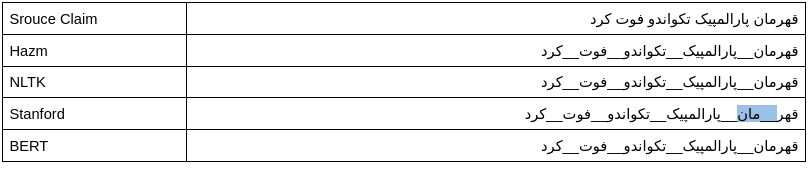
\includegraphics[width=16cm]{statistics/tokenizer/3.png} }}%
	\caption{Comparison performance of \textit{Hazm}, \textit{Stanford}, \textit{NLTK} and \textit{BERT} tokenizers.}%
	\label{fig:tekenres}%
\end{figure}

	Besides, the duration of tokenizing for each tokenizer is compared in figure \ref{fig:tokentime}. While \textit{Hazm} is the fastest words tokenizer among evaluated algorithms, \textit{Stanford} tokenizer lasts significantly longer. According to all pieces of evidence, \textit{Hazm} tokenizer is the best tokenizer for this task.

\begin{figure}%
	\centering
	{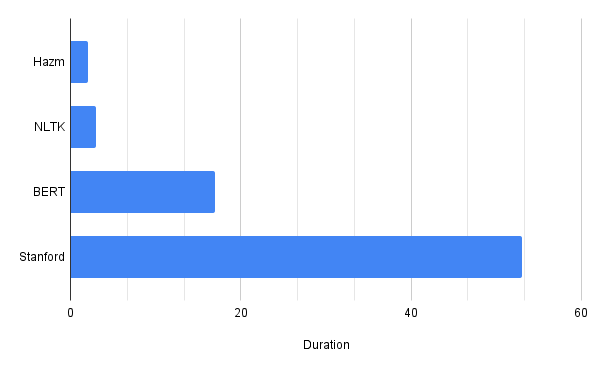
\includegraphics[width=12.5cm]{statistics/tokenizer/duration.png} }
	\caption{Comparison duration of tokenizing algorithm on \cite{stance_persian} dataset.}%
	\label{fig:tokentime}%
\end{figure}

\section{Stop-Words}
After preprocessing tokens, stop-words will be removed from the tokens. Firstly, the same stop-words list which has been used by \cite{stance_persian} was used in the project. After reviewing preprocessed corpus, it was hard to infer the stance from text pieces. So we chose stop-words carefully in a way not to lose refuting or supporting expressions.

Kharazi\footnote{\label{fn:kharazi}github.com/kharazi/persian-stopwords} has classified Persian stop-words into verbal, nonverbal, and short. Verbs carry valuable information in news. Nonverbal stop-word class is a better choice to remove low-value words in this task. Besides, we added and removed some words from Nonverbal list to become suitable for the news context. 


The difference between the performance of these four sets of stop-words in addition to skipping removing stop-words (To have a fair comparison) is illustrated in figure \ref{fig:stopwords}. \cite{stance_persian} contains 1255 words which include wide a range of parts of speech. In contrast, NonVerbal\footnote{Gathered by \href{github.com/kharazi/persian-stopwords}{Kharazi}} stop words set includes 158 words and it doesn't support any verb. In the new version of stop-words, 18 stop words are removed from the Nonverbal set. This set is called \textit{shortened} and 82 new words are added. Finally, the \textit{Extended} version contains 233 words. To evaluate the performance of each stop-words sets, all desired features with Tf-iDF as word representation after removing particular stop words are fed into an SVM (\cite{svc}) model.

It can be inferred from figure \ref{fig:stopwords} that the list of stop-words which is used by \cite{stance_persian} is ignoring valuable data and it is even better not to remove stop-words from the corpus. Nonverbal stop-words achieve higher accuracy on stance detection. Through, whether removing or adding words from Nonverbal (\textit{shortened} version) didn't improve results. Altogether, Nonverbal list of stop-words, performs the best in this task. 
Then all remaining tokens will be concatenated with a space character and considered as prepossessed and clean corpus.

\begin{figure}%
	\centering
	{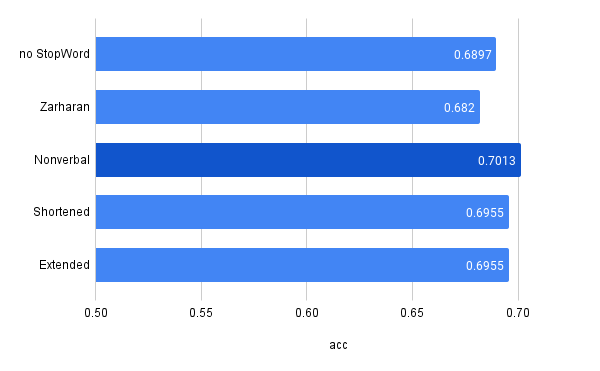
\includegraphics[width=12.5cm]{statistics/AccuracyScore.png} }
	\caption{Comparison accuracy of SVM model with different configuration of stop words.}%
	\label{fig:stopwords}%
\end{figure}

\section{Word Representation}
As a baseline, three different Bag-of-word (\cite{bow}), TF-iDF (\cite{tfidf}), and Word-to-Vector (\cite{word2vec}) algorithms are evaluated against each other. More details are explained in section \ref{lr:wordrep}.

In this project, FastText\footnote{fasttext.cc} Word2Vec model is used with vector lengths equal to 300 which is trained on the Persian Wikipedia website. For both TF-iDF and BoW n-gram range is set from 1 to 2. 

BoW (\cite{bow}), TF-iDF, and Word2Vec (\cite{word2vec}) performances are compared by the SVM machine learning algorithm in the stance detection task. According to figure \ref{fig:wordrep} Tf-iDF performs the best in comparison to BoW and Word2Vec in order to represent words.
\begin{figure}%
	\centering
	{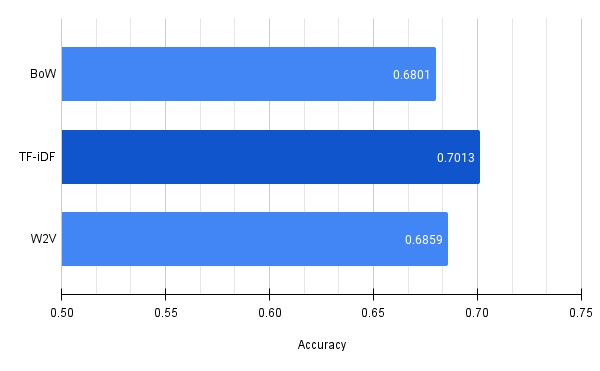
\includegraphics[width=12.5cm]{statistics/WordRep.png} }
	\caption{Comparison SVM model with Bow, TF-iDF and Word2Vec word representaion algorithms.}%
	\label{fig:wordrep}%
\end{figure}

\section{Predictors}
\label{sec:predictors}
Different combinations of calculated predictor are run to find out that which set of predictors performs better. Desired predictors are Similarity, RootDistance, IsQuestion, HasTwoParts and Polarity. In this Section, both SVM (\cite{svc}) and RandomForest (\cite{randomforest}) results are considered in evaluation to have a more accurate analysis. The similarity score is calculated by utilizing \textit{difflib}\footnote{docs.python.org/3/library/difflib.html} python library.


Firstly, both models are trained on the corpus representation by TF-iDF without any other predictor. Then, each predictor is added into TF-iDF vector to evaluate their effectiveness individually, and finally, all features together are fed to models. According to table \ref{tlb:predictors}, Similarity and ImportantWords have the highest positive effect respectively, on both accuracy (\ref{eq:acc}) and f1-score (\ref{eq:f1}). Similarity score has improved accuracy 15 to 17 percent and ImportantWords has improved SVM accuracy by almost 4 percent. Though, predictors such as IsQuestion, HasTwoParts, and Polarity don't have a significant effect on results, using them all together boost total accuracy and f1-score. 

Due to figure \ref{tlb:predictors}, using RootDistance, IsQuestion, and HasTwoParts individually decreases accuracy, so models are also trained with two other variations. Though IsQuestion, HasTwoParts, and polarity don't have a positive effect individually, using them with Similarity, ImportantWrods, and polarity boost accuracy. On the other hand, removing RootDistance from All predictors mode whether has a negligible effect or improves accuracy. 

According to previous comparisons and evaluation inferred from table \ref{tlb:predictors}, the best predictors to use for stance detection task is the combination of Similarity, ImportantWords, IsQuestion, HasTwoParts, and Polarity predictors in addition to TD-iDF as the corpus representer, altogether.

\begin{table}
	\centering
	\caption{Comparison of accuracy score and F1-score with different combinations of predictors for both SVM and Random Forest classifiers.}
	\setlength{\extrarowheight}{5pt}%
	\begin{tabular*}{350pt}{@{\extracolsep{\fill}}| l | l | l | l | l |}
		\hline
		\multicolumn{1}{|c|}{} & \multicolumn{2}{l|}{SVM} & 
		\multicolumn{2}{l|}{RandomForest}  \\ \cline{2-5} 
		
		\multicolumn{1}{|c|}{\multirow{-2}{*}{\begin{tabular}[c]{@{}c@{}}Predictors\\  Model\end{tabular}}}         & Acc.    & F1.    & Acc.    & F1.    \\ \cline{1-1}
		
		\hline \hline
		
		\multicolumn{1}{|c|}{TF-iDF only} & 51.83   & 51.90   & 52.79   & 54.00   \\ \cline{1-1}
		\hline
		+ Similarity      		& 66.85   & 66.71   & 68.78   & 67.88   \\ \cline{1-1}
		\hline
		+ Root Distance   		& 51.25   & 51.50   & 49.71   & 50.52   \\ \cline{1-1}
		\hline
		+ Important Words 		& 56.64   & 56.94   & 52.98   & 52.49   \\ \cline{1-1}
		\hline
		+ Is Question     		& 51.63   & 51.79   & 51.63   & 52.70   \\ \cline{1-1}
		\hline
		+ Has Two Parts   		& 51.83   & 51.90   & 50.28   & 50.87   \\ \cline{1-1}
		\hline
		+ Polarity        		& 52.21   & 52.50   & 52.40   & 53.25   \\ \cline{1-1}
		\hline
		+ All                   & 69.74   & 69.75  & 69.36   & 68.75   \\ \cline{1-1}
		\hline
		+ All - Root Distance   & 69.74   & 69.69   & \textbf{70.71}   & \textbf{70.28}   \\ \hline
		+ Similarity + ImportantWords   & 69.74   & 69.69   & 67.82  & 67.02  \\ \hline
	\end{tabular*}
	\label{tlb:predictors}
\end{table}

\section{Machine Learning}
\label{sec:ml}
In this section, each Gaussian Naive Bayes, SVM, Linear SVC, Random Forest, and Logistic Regression parameters are tuned on stance detection task with respect to chosen predictors in the previous section (\ref{sec:predictors}). In the next step, the performance of models is compared to each other.

\subsection{SVM}
In this project, We adopted SVC model implementation from \textit{scikit-learn}\footnote{scikit-learn.org/stable/modules/generated/sklearn.svm.SVC.html} python library is used in this project. \textit{class\_weight} parameter set to \textit{balanced} to compensate imbalanced data. Three SVM classifier tuned parameters  are Kernel, Regularization parameter (C) and degree of polynomial kernel. Evaluated kernels are RBF, Polynomial and Sigmoid. According to figure \ref{fig:svm}, Sigmoid works weak for this task. Each polynomial kernel behaves differently due value of the regularization parameter. Polynomial with degrees 2 and 3 perform better than 1 and 4. Linear polynomial may be so simple and SVM is not good enough to classify stance with a polynomial with degree 4. RBF, Polynomial degree 3 behave similarly due to the regularization parameter changes. 

The best configuration for SVM classifier is using RBF as the kernel with regularization parameter equal to 2.5 confirming figure \ref{fig:svm}. Learning procedure and details of each model training exist in this project GitHub repository\footnote{Different SVM configuration training details \href{https://github.com/mahsaghn/stance\_detection/tree/main/selected\_outputs/machinelearning/svm}{[here]}.}.

\begin{figure}% 
	\centering
	{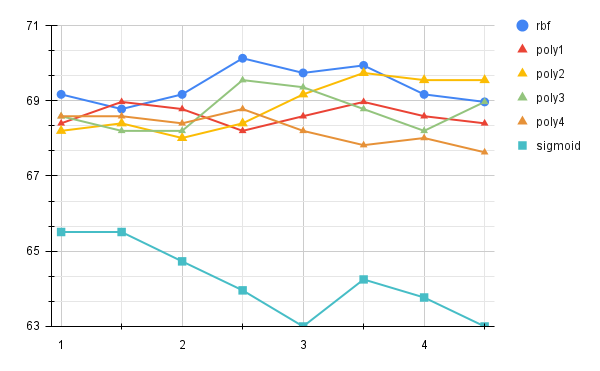
\includegraphics[width=12.5cm]{statistics/svm.png} }
	\caption{Tuning SVM model parameters with TF-iDF representation algorithms}%
	\label{fig:svm}%
\end{figure}

\subsection{Linear SVC}
Linear Support Vector Machine Classifier algorithm, loss function and Regularization parameters are tuned with penalty equals to \textit{l2}. Figure \ref{fig:linearsvm} illustrates comparison between linear svm models with loss functions equal to Hinge or Squared Hinge, and tuned SVM algorithm. Hinge loss function has scored better performance than Squared Hinge. When Squared Hing is used as loss function, as the Regularization parameter increases, accuracy score decrease. Though Regularization parameter don't have significant effect on accuracy score when loss is equal to Hinge. In conclusion, due to figure \ref{fig:linearsvm} Best configuration is for Hinge loss and Regularization parameter equals to 1.0. 
\begin{figure}% 
	\centering
	{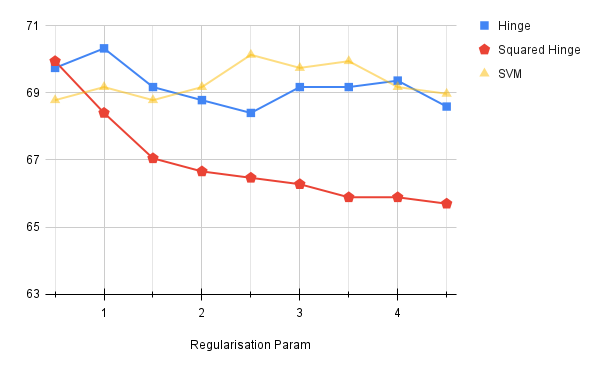
\includegraphics[width=12.5cm]{statistics/linearsvm.png} }
	\caption{Tuning LinearSVC model parameters with TF-iDF representation algorithms.}%
	\label{fig:linearsvm}%
\end{figure}
\subsection{Random Forest}
In this project, implemented Random Forest algorithm from \textit{scikit-learn}\footnote{scikit-learn.org/stable/modules/generated/sklearn.ensemble.RandomForestClassifier.html} python library is used. Three parameters of \textit{max\_features} (Maximum number of features allowed to use for each tree), \textit{estimator} (Number of decision trees), and \textit{criterion} (Algorithm to measure the quality of splits in nodes) are tuned for the desired task.

Figure \ref{fig:randomforest} illustrates the effect of the number of trees in the forest on accuracy among different configuration. The average accuracy score of models increases by adding more trees into the forest. Besides, \textit{gini} algorithm performs better than \textit{entropy} to measure the quality of splits. Also, three different upper bounds are considered for number of features when looking for a split. No boundary, \textit{sqrt} of total features and \textit{log2} of total feature. According to figure \ref{fig:randomforest} don't apply any boundary leads to better accuracy on average. Furthermore, as the boundary gets tighten average performance decreases. 

The best configuration for Random Forest machine learning model in this task is using \textit{gini} algorithm to evaluate splitting quality, not applying any boundary on the number of features and having 125 decision trees in the forest. 
\begin{figure}% 
	\centering
	{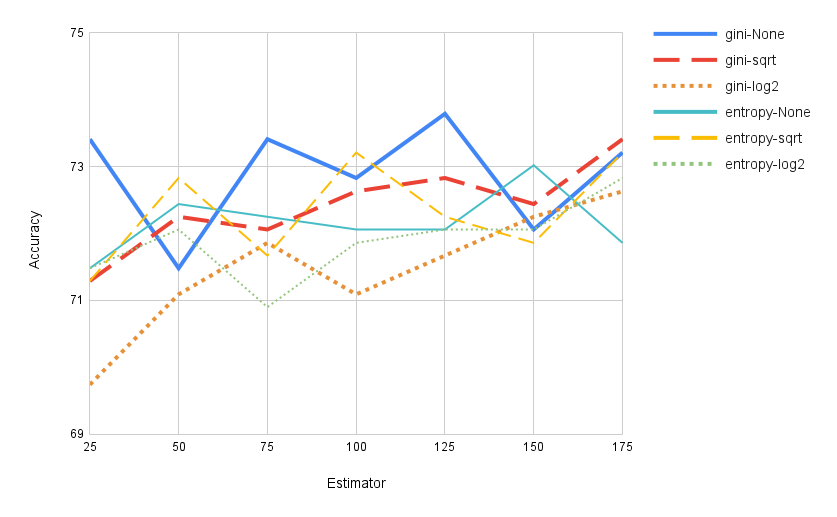
\includegraphics[width=12.5cm]{statistics/randomforest.png} }
	\caption{Random Forest machine learning model different configuration on stance detection task. Type of line presents type of the boundary applied on each model. Solid line, dash line and doted line stands for no boundary, sqrt of total feature and log2 of total feature respectively.}%
	\label{fig:randomforest}%
\end{figure}
\subsection{Logistic Regression}
We also adopted the Logistic Regression algorithm from the \textit{sckiti-learn}\footnote{scikit-learn.org/stable/modules/generated/sklearn.linear\_model.LogisticRegression.html} python library. Many experiments are designed to evaluate behavior of Logistic Regression models. 	 \textit{Elasticnet} (Equation \ref{eq:logisel}) penalty algorithm which is used in penalization procedure, used for \textit{saga} solver and \textit{l2} penalty algorithm is used for \textit{sag}, \textit{lbfgs}, and \textit{newton-cg} solvers. 

\textit{Elasticnet} has a $\rho$ parameter which determines the portion of using $l1$ to $l2$ penalty in \textit{saga} solver. Figure \ref{fig:logistic1} illustrate the effect of $\rho$ values from $0$ to $0.9$ on the accuracy of stance detection. Besides, models with a regression parameter from $0.5$ to $4.5$ are evaluated from the determined $\rho$ range. It can be inferred from figure \ref{fig:logistic1} that $\rho$ parameter doesn't have a significant effect on the accuracy of the model. While regression parameter between $1$ and $2.5$ clearly results in higher accuracy rather than external range. It can be also inferred from figure \ref{fig:logistic2} which illustrates the effect of the regression parameter on stance classification accuracy. Models with different values of $\rho$ behave similarly and best performances happen when regression parameter is between $1$ and $2.5$.  
\begin{figure}% 
	\centering
	{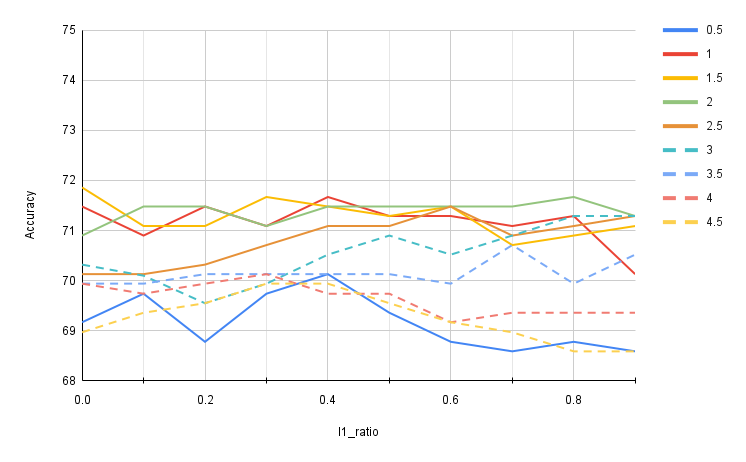
\includegraphics[width=12.5cm]{statistics/logistic_elastic1.png} }
	\caption{Effect of $\rho$ parameter of \textit{elasticnet} penalty on stance detection task.}%
	\label{fig:logistic1}%
\end{figure}
\begin{figure}% 
	\centering
	{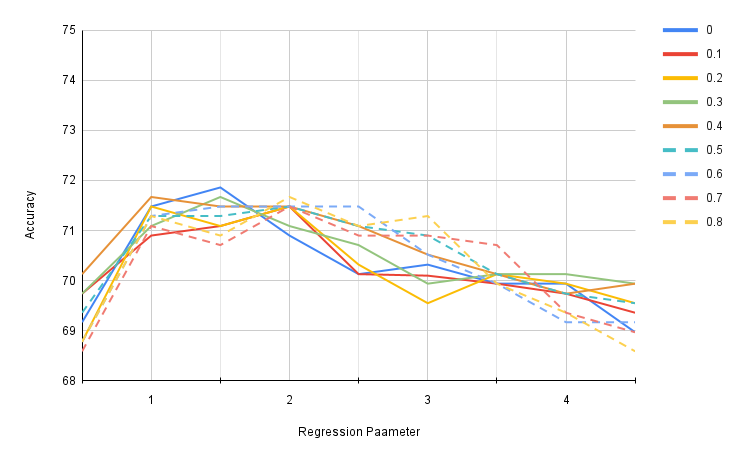
\includegraphics[width=12.5cm]{statistics/logistic_elastic2.png} }
	\caption{Effect of regression parameter of \textit{elasticnet} penalty on stance detection task.}%
	\label{fig:logistic2}%
\end{figure}

Another variant of Logistic Regression setup is to use $l2$ penalty with desired solver algorithms. Figure \ref{fig:logistic3} compares best \textit{saga} solver with \textit{sag}, \textit{lbfgs}, and \textit{newton-cg}. The Logistic Regression with \textit{lbfgs} solver and regression parameter equals 1.5 has recorded the highest accuracy. 
\begin{figure}% 
	\centering
	{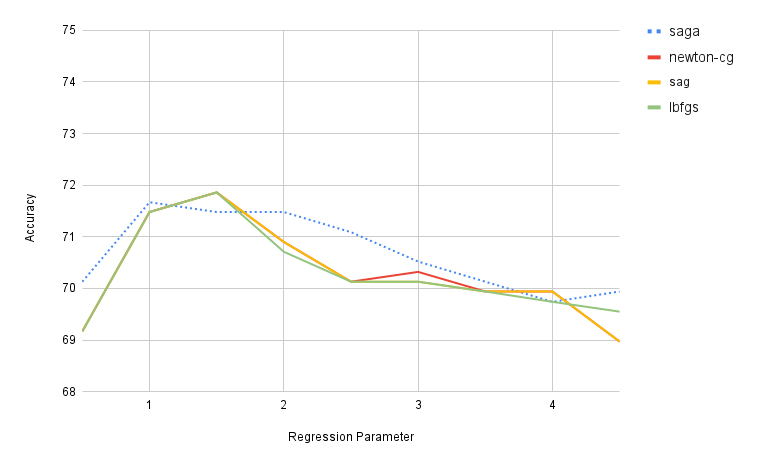
\includegraphics[width=12.5cm]{statistics/logistic1.png} }
	\caption{Comprasion of Logistic Regression machine learning models.}%
	\label{fig:logistic3}%
\end{figure}

\subsection{Comparison}
In previous sections parameters of each SVM, LinearSVC, Random Forest, and Logistic Regression models are tuned. In this section models with desired parameters have run 5 times each to have more reliable results and comparison. Average accuracy and highest accuracy recorded in tuning phase, compared in figure \ref{fig:all}. The highest achievable accuracy with machine learning models to classify the stance of a claim towards the headline of a news article is 74.01\%.
\begin{figure}% 
	\centering
	{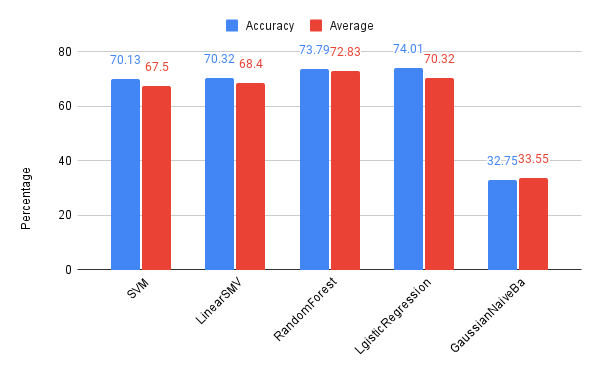
\includegraphics[width=12.5cm]{statistics/machinlearning.png} }
	\caption{Comparison SVM model between Bow, TF-iDF and Word2Vec word representation algorithms.}%
	\label{fig:all}%
\end{figure}
\section{Dataset Balancing}
As mentioned in section \nameref{sec:dataset}, Figure \ref{fig:datacom}, the number of samples in dataset classes was imbalanced. So oversampling should be performed in classes except for the majority class.
In \cite{stance_persian} minority class forms only 7.4\% of data (Figure \ref{fig:datacom}).
 All oversampling methods are evaluated against each other in this project and utilized from the oversampling package of \textit{imblearn} \footnote{imbalanced-learn.org/stable/references/over\_sampling.html} python library. 

\begin{figure}%
	\centering
	\subfloat[\centering Artcile to Claim]{{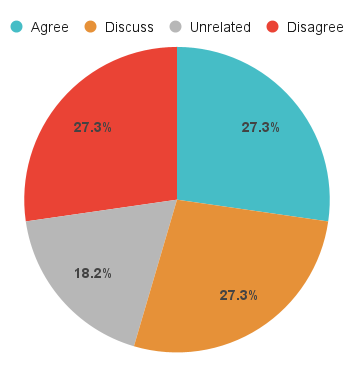
\includegraphics[width=6cm]{statistics/stance/a2c_b1.png} }}%
	\qquad
	\subfloat[\centering Headline to claim ]{{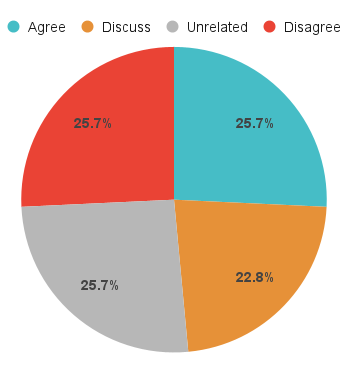
\includegraphics[width=6cm]{statistics/stance/h2c_b1.png} }}%
	\caption{Comparison between article-to-claim and headline-to-claim labels, samples distribution in \cite{stance_persian} dataset, after extending by \cite{parsfever} .}%
	\label{fig:datab1}%
\end{figure}



Firstly, ADASYN, SMOTE, SVMSMOTE, BorderLineSmote, and RandomOverSampler oversampling methods are applied on the \cite{stance_persian} dataset. In ADASYN algorithm, the number of nearest neighbors to generate a new sample is set to 9\footnote{imbalanced-learn.org/stable/references/generated/imblearn.over\_sampling.ADASYN.html}. Each method is evaluated against five desired machine learning models. Red series in figure \ref{fig:balanc} stands for the accuracy of models, associated with the \cite{stance_persian} dataset. LinearSVC, LogisticRegresion, and GaussianNaibeBayes are not compatible with any oversampling method. Though, ADASYN oversampling method has increased these two model accuracy $5$ percent on average.


In the second step, the dataset is extended by the ParsFever (\cite{parsfever}) dataset. Though the number of samples is increased accuracy is obviously decreased, but the GaussianNB model. This may happen that data sources from each dataset are totally different and headlines in ParsFever are much longer than the \cite{stance_persian} dataset.
\begin{figure}% 
	\centering
	{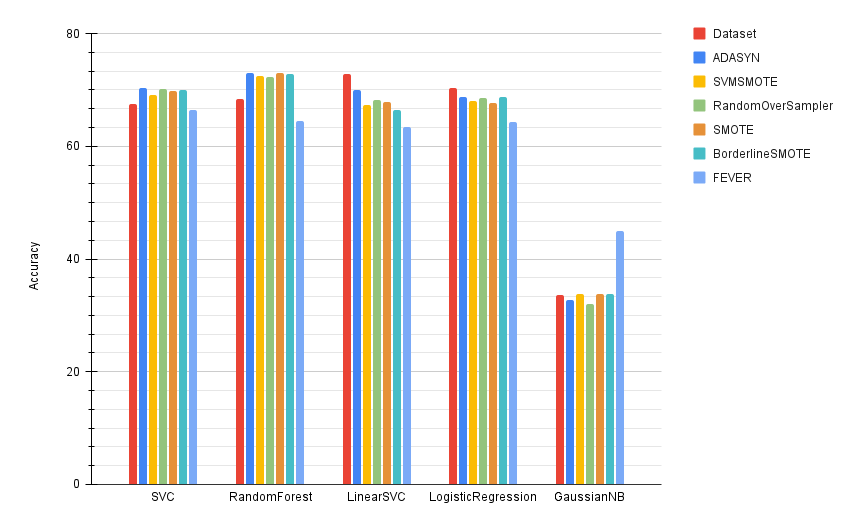
\includegraphics[width=14.5cm]{statistics/balancing.png} }
	\caption{Comparison SVM model with Bow, TF-iDF and Word2Vec word representation algorithms.}%
	\label{fig:balanc}%
\end{figure}

\section{Deep Learning}

\label{sec:dl}
A Pre-trained BERT-based model is used at the top of the model, then two Dense layers and finally a Dense including 4 neurons to classify stance is considered for the end-to-end system. The input of our deep learning models is \textit{input ids}, \textit{token type ids}, and \textit{attention mask}.
BERT (\cite{bert}), ParsBERT \cite{parsbert}, and ALBERT (\cite{albert}) models are substitute with Pretrained ML model in figure \ref{fig:dlschm}. Each epoch lasts about 26 seconds in the training procedure. Figure \ref{fig:deep} illustrates the model training procedure. In comparison to machine learning models, the deep learning model has boosted the accuracy of headline-to-claim stance detection by 10 percent. 

The BERT-based model has been learned for 20 epochs. Validation loss has been stated to increase since epoch 11 and validation accuracy hasn't changed considerably then. Best validation accuracy has converged on $80.92\%$ on the headline-to-claim dataset. 

The ParsBert-based model has been learned for 20 epochs. Best validation accuracy has converged on $81.11\%$ on the headline-to-claim dataset. In comparison to the machine learning algorithm, deep learning algorithm has enhanced about $10\%$ accuracy. Besides, the loss score has converged on a lower score than BERT-based model.

Though, the best recorded ALBERT language model on 20 epochs is at most $70.52\%$ on accuracy score. Figure \ref{fig:deep}, parts (e) and (f) is illustrated the training procedure.

Among these three alternatives of the BERT algorithm, PasrBERT based model has recorded the best accuracy score with $85.48\%$ accuracy on stance prediction.  
\begin{figure}%
	\centering
	\subfloat[\centering]{{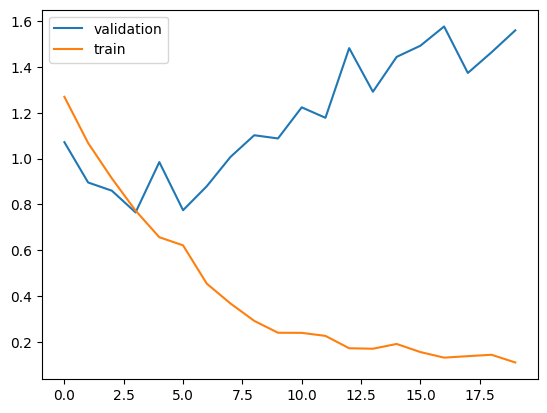
\includegraphics[width=6cm]{statistics/deep/bert_loss.png} }}%
	\qquad
	\subfloat[\centering]{{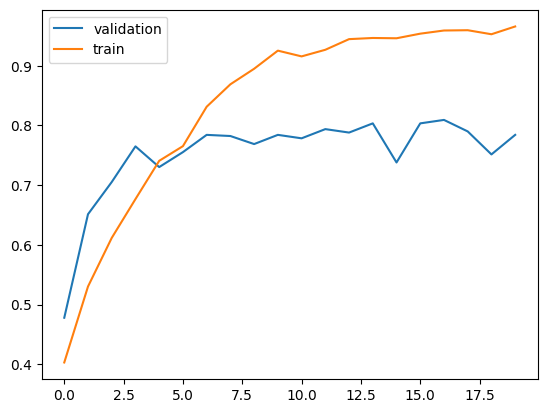
\includegraphics[width=6cm]{statistics/deep/bert_acc.png} }}%
	\qquad
	\subfloat[\centering]{{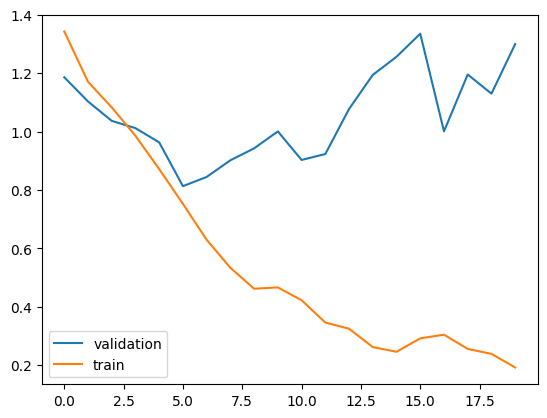
\includegraphics[width=6cm]{statistics/deep/parsbert_loss.png} }}%
	\qquad
	\subfloat[\centering]{{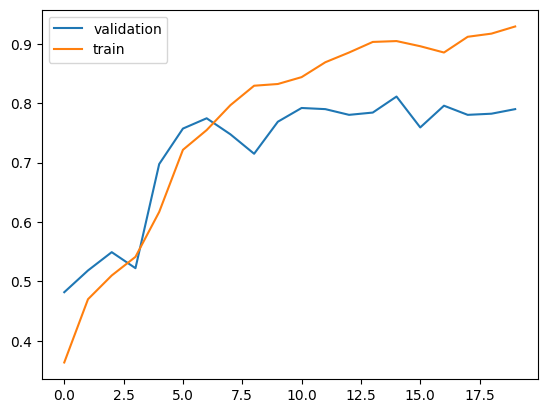
\includegraphics[width=6cm]{statistics/deep/parsbert_acc.png} }}%
	\qquad
	\subfloat[\centering]{{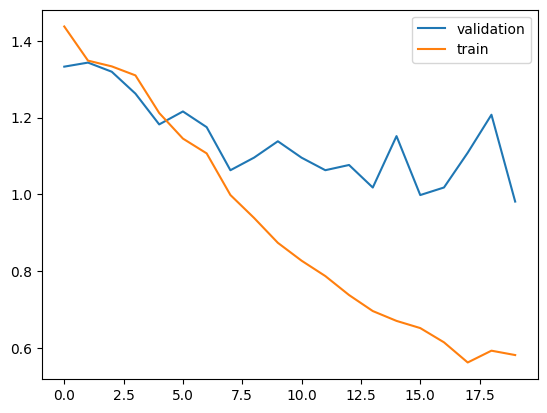
\includegraphics[width=6cm]{statistics/deep/albert_loss.png} }}%
	\qquad
	\subfloat[\centering]{{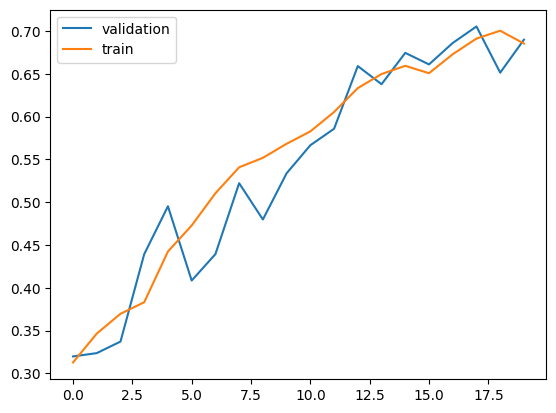
\includegraphics[width=6cm]{statistics/deep/albert_acc.png} }}%
	
	
	\caption{Deep learning procedure on the headline-to-claim stance detection task. Left figures illustrate loss score and right figures illustrate accuracy score of train and test data during the training procedure. (a, b) Pre-trained language model based on Google's BERT (\cite{parsbert}) on Persian corpus (c, d) Pre-trained monolingual language model based on ParsBERT (\cite{parsbert}) on Persian corpus. (e, f) Pre-trained language model based on ALBERT (\cite{albert}) on Persian corpus}%
	\label{fig:deep}%
\end{figure}

\begin{table*}[t]
	\centering
	\small
	\caption{Comparison of headline-to-claim stance detection models.}
	\def\arraystretch{1.3}%
	\setlength{\extrarowheight}{5pt}%
	\begin{tabular}{|c|c|c|c|c|}
		\hline{Model} & {Precision} & {Recall} & {F1} & {Accuracy}\\
		\hline \hline
		{SVM+ADASYN} & {69.63} & {69.15} & {69.38} & {70.32}\\
		\hline
		{RandomForest+ADASYN} & {71.24} & {69.14} & {70.17} & {73.02}\\
		\hline
		{BERT} & {81.65} & {80.69} & {81.16} & {80.92}\\
		\hline
		{ParsBERT} & {84.67} & {79.42} & {81.96} & {81.11}\\
		\hline
		{ALBERT} & {75.75} & {64.09} & {69.43} & {70.52}\\
		\hline
		{ParsBERT+ADASYN} & {84.96} & {85.64} & {85.29} & {\textbf{85.48}}\\
		\hline
	\end{tabular}
	\label{tbl:allstance}
\end{table*}


\section{Article to Claim}

Best stance detection models on both machine learning and deep learning models are evaluated on article-to-claim task. The length of 400 characters is considered for the maximum length of article content. Table \ref{tbl:allstance} show those models performance on both headline-to-claim and article-to-claim task. Using ADASYN oversampler and ParsBERT as the pre-trained language leads to our best results on both headline-to-claim and article-to-claim models. We achieved 80.62\% accuracy score on the article-to-claim task. Out experiments on article-to-claim achieved a lower score than the headline-to-claim task because inferring from longer text is a harder task for the model.  

\begin{table*}[t]
	\centering
	\small
	\caption{Comparison between article-to-claim machine learning and deep learning models.}
	\def\arraystretch{1.3}%
	\setlength{\extrarowheight}{5pt}%
	\begin{tabular}{|c|c|c|c|c|}
		\hline
		{} & \multicolumn{2}{c|}{Headline to claim} &  \multicolumn{2}{c|}{Article to claim}\\
		\hline 
		{Model} & {F1} & {Accuracy} & {F1} & {Accuracy}\\
		\hline	\hline
		{SVM+ADASYN} & {69.38} & {70.32} & {65.18} & {64.49}\\
		\hline
		{ParsBERT} & {81.96} & {81.11} & {78.00} & {78.32}\\
		\hline
		{ParsBERT+ADASYN} & {85.29} & \textbf{{85.48}} & {80.29} & \textbf{{80.62}}\\
		\hline
	\end{tabular}
	\label{tbl:a2c}
\end{table*}

\section{Fake News}
The best BERT-based model for headline-to-claim and article-to-claims are considered for this part. These model prediction base on 4 news articles are concatenated with features which are described in section \ref{sec:fakenews}. Then the overall vector is feed to a three-layer MLP model as the classifier. ADASYN oversampling method is also used to deal with imbalanced classes. Figure \ref{fig:fakenews} illustrates the training procedure before oversampling and after oversampling the dataset. After oversampling, the trained model accuracy has converged to 99\%, while before oversampling model stops at $90.41\%$. According to figure \ref{fig:fakenews}, after adding oversampled samples, at first iterations, it is harder for the model to decrease the loss score on the train set and loss score convergent takes a longer time. Though after balancing the dataset (Figure \ref{fig:fakenews}, part (a)), the value of loss score has converged 0.2 lower than the original dataset (Figure \ref{fig:fakenews}, part (c)).

\begin{figure}%
	\centering
	\subfloat[\centering]{{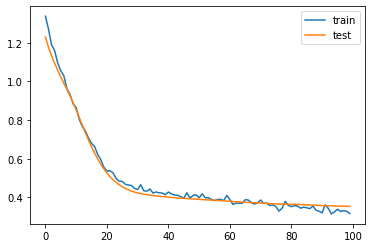
\includegraphics[width=6cm]{statistics/fakenews/dataset/loss.png} }}%
	\qquad
	\subfloat[\centering]{{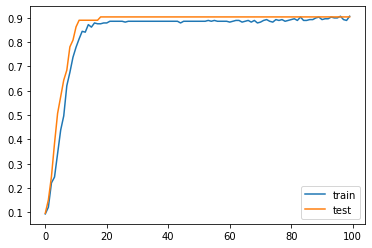
\includegraphics[width=6cm]{statistics/fakenews/dataset/acc.png} }}
	\qquad
	\subfloat[\centering]{{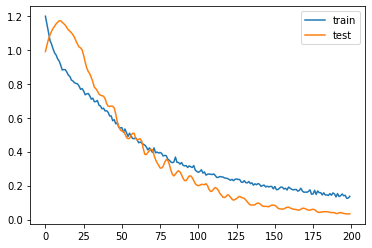
\includegraphics[width=6cm]{statistics/fakenews/oversampled/loss.png} }}%
	\qquad
	\subfloat[\centering]{{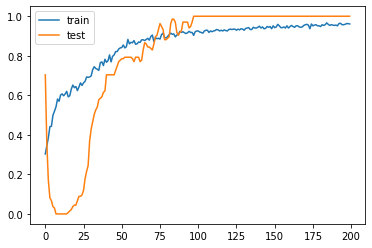
\includegraphics[width=6cm]{statistics/fakenews/oversampled/acc.png}}}
	\caption{Left figures illustrate loss score and right figures illustrate accuracy score of train and test data during training procedure for each iteration. 
		(a, b) Training procedure on fake news detection model trained on the \cite{stance_persian} dataset.
		(c, d) Training procedure on fake news detection model trained on oversampled \cite{stance_persian} dataset by ADASYN (\cite{adasyn}) algorithm.}%
	\label{fig:fakenews}%
\end{figure}